\label{sec:evaluation}

We perform our evaluations on a quiescent 8-core system
(dual processor with 4 cores), and 8GB of RAM. Each pro-
cessor is a 4-core 64-bit Intel Xeon running at 2.33 Ghz
with a 4MB L2 cache. Note that those applications are generated
for a 32bit environment using ``-m32''. 

All performance data in this section are the average of 10 times running, with the maximum value and minimum value are 
excluded here.

In this section, we are going to answer the following questions:
\begin{itemize}
\item How effective is Sheriff to find false sharing problems?
	  %% How many false sharing problems can be found by Sheriff? Show some small examples.
	  %% The atucal effect of Sheriff to find the false sharing problems in actual applications.
\item How is the performance of Sheriff comparing to that using pthreads library.
\item What can affect the performance of Sheriff?
\end{itemize}

\subsection{Effectiveness}
This section are trying to valify whether Sheriff can be used to find false sharing problems both in 
our designed test cases and in actual applications. 
%Also, we are trying to verify whether Sheriff has false positives (mistakely report non-false sharing problems)
%and whether Sheriff has a lot of false negatives (miss some false sharing problems). 

\subsubsection{Micro-benchmarks}
According to our discussion in Section~\ref{overview:target}, 
Sheriff can be used to detect false sharing problems including false sharing, pseudo sharing. 
The first step of evaluation is to design some test cases which examplify these problems and try to verify whether Sheriff
can be used to detect those problems. To be compared, we also list the corresponding results of PTU.
\begin{figure}[!t]
\begin{lstlisting}
int count1 = 0; int count2 = 0;
void * thread1(void * param) {
  for(i = 0; i < COUNT_NUM; i++)
    count1++;		
}
void * thread2(void * param) {
  for(i = 0; i < COUNT_NUM; i++)
    count2++;       
}
\end{lstlisting}
\caption{benchmark1(falsesharing)   
\label{fig:benchmark1}}
\end{figure}

\begin{figure}[!t]
\begin{lstlisting}
int count[CORE_NUM];
void * thread(void * param) {
  int tid = (int)param;
  for(i = 0; i < COUNT_NUM; i++)
    count[tid]++;       
}
\end{lstlisting}
\caption{benchmark2(pseudosharing)
\label{fig:benchmark2}}
\end{figure}

\begin{figure}[!t]
\begin{lstlisting}
int count = 0; 
void * thread(void * param) {
  for(i = 0; i < COUNT_NUM; i++) 
    count++;       
}
\end{lstlisting}
\caption{benchmark3(truesharing)
\label{fig:benchmark3}}
\end{figure}

\begin{figure}[!t]
\begin{lstlisting}
int count1 = 0; int count2 = 0;
void * thread1(void * param) {
  for(i = 0; i < COUNT_NUM; i++)
    count1++;       
}
void * thread2(void * param) {
  for(i = 0; i < COUNT_NUM; i++)
    count2++;       
}
int main() {
	spawn(&tid[0], thread1); join(tid[0]);
	spawn(&tid[1], thread2); join(tid[1]);
}
\end{lstlisting}
\caption{benchmark4(noninterleaving-falsesharing).
\label{fig:benchmark4}}
\end{figure}

\begin{figure}[!t]
\begin{lstlisting}
int * pcount1; int * pcount2;
void * thread1(void * param) {
  for(i = 0; i < COUNT_NUM; i++)
    pcount1[0]++;       
}
void * thread2(void * param) {
  for(i = 0; i < COUNT_NUM; i++)
    pcount2[1]++;       
}
int main() {
	pcount1 = malloc(16);
    spawn(&tid[0], thread1);  join(tid[0]); 
    free(pcount1);
	// New allocation here.
	pcount2 = malloc(16);
    spawn(&tid[1], thread2); join(tid[1]);
}
\end{lstlisting}
\caption{benchmark5(heap caused false negative).
\label{fig:benchmark5}}
\end{figure}

\begin{table}
\centering
\begin{tabular}{|l|l|l|l|}
\hline
{\bf \small Microbenchmark} & {\bf \small Perf-Sensitive} & {\bf \small Sheriff } & {\bf \small PTU } \\
 & {\bf \small False Sharing} & & \\
\hline

\small \textbf{benchmark1} & True & True & True\\
\small \textbf{benchmark2} & True & True & True\\
\small \textbf{benchmark3} & False & False & False\\
\small \textbf{benchmark4} & False & False & True\\
\small \textbf{benchmark5} & False & False & True\\
\hline
\end{tabular}
\caption{False sharing detecting results using PTU and Sheriff. 
``True'' - tool will report false sharing. ``False'' - tool won't report false sharing. 
\label{table:microbenchmarks}}
\end{table}

Results can be seen in Table~\ref{table:microbenchmarks}. We can see that Sheriff can report those 
false sharing (Fig.~\ref{fig:benchmark1}) and pseudo sharing (Fig.~\ref{fig:benchmark2}) problems sucessfully. 
Clearly, it is better not to report that on benchmark3(Fig.~\ref{fig:benchmark3}), 
benchmark4(Fig.~\ref{fig:benchmark4}) and benchmark5(Fig.~\ref{fig:benchmark5}). 
But PTU can wrongly report a false sharing for benchmark4 and benchmar5.
Sheriff can successfully avoid these noisy information to programmer 
thus can save much time to rule out those false positives.
Note that benchmark5 (Fig.~\ref{fig:benchmark5}) is an typical false positives 
caused by dynamic heap object. 
Two different allocations happened to be in the same placement. 
To the best of our knowledge, Sheriff is the first tool 
which can avoid this type of false positives since Sheriff 
cleanups invalid counting information (after \texttt{free(pcount1)})
and focuses on interleaving writes only.
%%%%%%%%%%%
%%% Whether we should add the pseudo code here.
%%%%%%%%%%%%
\subsubsection{Actual Applications}
\label{effect-application}
In order to verify whether Sheriff can be used to detect some false sharing problems in actual applications,
we run Sheriff against phoenix~\cite{phoenix-hpca} and PARSEC~\cite{parsec} benchmark suite.

We used the \textbf{simlarge} input for all applications of PARSEC. 
For Phoenix, we choose some correpspoinding parameters in 
order to run for sufficient time. 
There are some benchmarks that we cannot run on Sheriff caused by compilation error or runtime error:
\texttt{raytrace}, \texttt{vips} have some compilation errors and \texttt{x264}, \texttt{bodytrack}, \texttt{facesim}
have running problems. Thus, we haven't listed the results about these benchmarks here. 

%%%%%%%%%%%%%%%%%%%%%%%%%%%%%%%%%%%%%%%%%%%%%%%%%%%%%%%%%%%%%%%%%%%%%%%%%%%%%%%%%%%%%%%%%%%%%%
%%%%%% Use a table to listed some data about benchmarks and description of these benchmarks.
%%%%%% List how many false sharing objects are reported, how many objects are false sharing problems. 
%%%%%% How many commits inside, how many pages are written totally, how many allocations are invoked. 
%%%%%% Footprint of those protected pages, shared pages. 
%%%%%%%%%%%%%%%%%%%%%%%%%%%%%%%%%%%%%%%%%%%%%%%%%%%%%%%%%%%%%%%%%%%%%%%%%%%%%%%%%%%%%%%%%%%%%%
According to our experiments, Sheriff have found that 4 benchmarks (of 16 total benchmarks) 
have the false sharing problems inside. 
In \texttt{reverse\_index} and \texttt{word\_count}, different threads are trying to 
modify the same heap object. The pseudo code
for these two benchmarks are listed in Fig.~\ref{fig:reverseindex}. 
We can use thread-local copy to avoid the false sharing problem here; each thread can modify a temporary variable
first and then modify the global \texttt{use\_len} in the end of thread. 
\begin{figure}[!t]
\begin{lstlisting}
int * use_len;
void insert_sorted(int curr_thread) {
   ......	
   // After finding a new link
   (use_len[curr_thread])++;
   ......	
}
\end{lstlisting}
\caption{\texttt{reverse\_index} example. Here different threads 
can modify the same \texttt{use\_len} array when
there is a new link found. 
\label{fig:reverseindex}}
\end{figure}

\texttt{Linear\_regression} false sharing problem is a little different (see Fig.~\ref{fig:linear_regression}. 
Two different threads are writing on the 
same cache line when the structure \texttt{lreg\_args} is not cache line aligned. This problem can
be avoided easily by padding the structure \texttt{lreg\_args}.
\begin{figure}[!t]
\begin{lstlisting}
struct {
  long long SX;
  long long SY;
  long long SXX;
  ......
} lreg_args;
void *lreg_thread(void *args_in) {
  struct lreg_args * args = args_in;
  for(i = 0; i < args->num_elems; i++) {
    args->SX  += args->points[i].x;
    args->SXX += args->points[i].x 
			   * args->points[i].x;
  }
  ......	
}
\end{lstlisting}
\caption{\texttt{linear\_regression} false sharing example code. 
In the creation of thread, each thread will be passed in a different
address (\texttt{struct lreg\_args}) and each thread can work on its corresponding \texttt{args\_in}. 
But unforunately, the size of \texttt{struct lreg\_args} is not cach line aligned (52 bytes) and that
can cause two different threads are writing on the same cache line simultaneously. 
\label{fig:linear_regression}}
\end{figure}

False sharing problem detected in \texttt{streamcluster} (one of PARSEC benchmark) is something like the false 
sharing problem in \texttt{linear\_regression}; two different threads are writing on the same cache line. 
But the reason to cause that is different. In fact, author tries to avoid the false sharing
problems and make every stride multiple times of cache line size. But the default cache line 
size is 32 bytes, which is different with the actual physical cache line size that we are used in
evaluation. Our cache line size is 64 bytes. By simply setting the \texttt{CACHE\_LINE} macro to 64 bytes in order 
to avoid false sharing problem completely. 

The performance about these 4 benchmarks are listed in Table~\ref{table:perfafterfix}. 
\begin{table}
\centering
\begin{tabular}{|l|r|r|r|r|}
\hline
{\bf \small Benchmark} & {\bf \small Old} & {\bf \small New} & {\bf \small Speedup} & {\bf \small Updates}\\
& (s) & (s) & &(Mega)\\
\hline
\small \textbf{linear\_regression} & 9.116 & 0.89 & 1024.3\% & 1323.6\\
\small \textbf{reverseindex} & 5.449 & 5.427  & 100.41\% & 0.4\\
\small \textbf{word\_count} & 2.188 & 2.151 & 101.72\% & 0.3\\
\small \textbf{streamcluster} & 2.825 & 2.501 & 112.95\% & 28.7\\
\hline
\end{tabular}
\caption{Performance data for 4 false sharing benchmarks. 
``Old'' column shows the runtime (s) before we fix the false sharing problem 
and ``New'' column shows the runtime (s) after fix. 
All data are got based on the same pthreads library. 
``Updates'' shows how many Maga updates (totally) on false sharing related cache lines. 
\label{table:perfafterfix}}
\end{table}

In this table, we compare the performance before and after the fix of false sharing problems.
Then we list the speedup by fixing the false sharing problem. 
To exaplan why there are much difference in performance improvement, we also 
modify the code to get all possible updates caused by these false sharing objects. 
Updates listed here should be the maximum possible interleaving writes of these objects, actual 
interleaving writes depending on actual conditions. 
Here, \texttt{reverse\_index} and \texttt{word\_count} doesn't have huge improvements even after we fixed 
the false sharing problems inside. That is because the global array's updation is 
not a very large number, for example, \texttt{reverse\_index} max possible interleaving updates is 0.416Mega times.
For \texttt{linear\_regression}, the number of updation is pretty large, about 1323.61Mega times. 
But we believe that this modification is necessary if benchmarks have a larger input or benchmark is 
going to running on NUMA architecture.

\subsubsection{Comparison between Sheriff and PTU}
\label{evaluation:comparison}
%%%%%%%%%%%%%%%%%%%%%%%%%%%%%%%%%%%%%%%%%%%%%%%%%%%%%%%%%%%%%%
%%%%% OUTPUT here %%%%%%%%%%%%%%%%%%%%%%%%%%%%%%%%%%%%%%%%%%%%
%%%%%%%%%%%%%%%%%%%%%%%%%%%%%%%%%%%%%%%%%%%%%%%%%%%%%%%%%%%%%%%
In order to show how effective Sheriff can find false sharing problems, we compare the results with PTU.
There are two reasons that we are choosing PTU for comparision. 
First, PTU is a comercial products of Intel which we believe it can represent the state of art to detect
false sharing problems.
Second, PTU is the only available tool for us and PTU provides detailed guidelines and manuals,
which can help us to use the tool.

We are focuses two things in this comparison.
\begin{itemize}
\item
How many items are reported by different tools?
\item 
How easy to find the actual false sharing problem according to output?
\end{itemize}

\par\vspace{3mm}
\noindent
\textbf{Reporting Items}
\par\vspace{3mm}
\noindent
For PTU, we list numbers of cache line having false sharing problems (marked with pink color
by tool) for simplicity. At actually, to decide one false sharing problem,  
user have to look at those accesses in every cache line. 
For Sheriff, we lists objects number reported by Sheriff.

\begin{table}
\centering
\begin{tabular}{|l|r|r|}
\hline
{\bf \small Benchmark} & {\bf \small PTU} & {\bf \small Sheriff}\\
 & {\# Cachelines} & {\# Objects}\\
\hline
\small \textbf{histogram} & 0 & 0 \\
\small \textbf{kmeans} & 1916 & 0 \\
\small \textbf{linear\_regression} & 5 & 1 \\
\small \textbf{matrix\_multiply} & 468 & 0\\
\small \textbf{pca} & 45 & 0 \\
\small \textbf{reverseindex} & N/A & 1 \\
\small \textbf{string\_match} & 0 & 0 \\
\small \textbf{word\_count} & 4 & 1\\
\hline
\small \textbf{blackscholes} & 0 & 0 \\
\small \textbf{canneal} & 1 & 0 \\
\small \textbf{dedup} & 0 & 0 \\
\small \textbf{ferret} & 0 & 0\\
\small \textbf{fluidanimate} & 3 & 0 \\
\small \textbf{freqmine} & 0 & 0 \\
\small \textbf{streamcluster} & 9 & 1\\
\small \textbf{swaptions} & 196 & 0\\
\hline
\small \textbf{Total} & 2647 & 4\\
\hline
\end{tabular}
\caption{Detection results of PTU and Sheriff. For PTU, we shows 
how many cache lines are marked as false sharing. For Sheriff,
we shows how many objects are reported by Sheriff (with interleaving writes larger than 100 times). 
%The column "False-negatives" shows possible false negatives of Sheriff which we got results 
%manually by check those cachelines with larger than 100 times reference showed in PTU. 
The item marked as "N/A" means PTU cannot show results caused by out-of-memory errors. 
\label{table:detection}}
\end{table}

From the results listed in Table~\ref{table:detection}, we can see that Sheriff needs much less manual effort
to check those false sharing problems. We have to check 2647 cache lines 
according to PTU (not including \texttt{reverse\_index}) but checking only 4 cache lines according to Sheriff.
Also, all false sharing reported by Sheriff are actually false shairng problems. 

Several reasons can cause this difference. 
First, Sheriff reduce all false positives, this can reduce the number of reporting items greately. 
Second, Sheriff only reports those objects with interleaving writes larger than one threshold
(currently 100 times, which can be set easily), which significantly reduce the number of reporting.
Third, Sheriff reports corresponding objects instead of cache lines, which can also help to reduce the
reporting number too if one object covers multiple cache lines. 
%Readers wonder whether Sheriff misses some critical false sharing problems? 
\par\vspace{3mm}
\noindent
\textbf{Easiness to locate problem}
\par\vspace{3mm}
\noindent
Sheriff can precisely locate false sharing problems, which is easy to find the problems. 
For a global object, Sheriff can output global objects's name and size information. 
For a heap object, Sheriff can precisely tell the call site to allocate one object then it is easy
for programmer to find the problem caused by one object. 
Here, we are using the benchmark \texttt{word\_count} (one of Phoenix benchmark) as one example.

Sheriff can output like this:
\begin{verbatim} 
1th object, cache interleaving writes 
13767 times(start as 0xd5c8e140). 
Object start 0xd5c8e160, len 32. 
It is a heap object with callsite:
callsite 0:./wordcount_pthreads.c:136
callsite 1:./wordcount_pthreads.c:441
\end{verbatim}

If we take a look at the line 136(\texttt{wordcount\_pthreads.c}), 
there is a memory allocation like this:
\begin{verbatim}
use_len=malloc(num_procs*sizeof(int));
\end{verbatim}

If we check the code about the usage of \texttt{use\_len} (simply search), 
then we can find a lot of usage about 
about this global pointer. 
\begin{verbatim}
use_len[thread_num]++;
\end{verbatim}

Now it is clear that different threads are modifying the same object (use\_len). 
Then it is easy to fix the problem by using the thread-local data copies~\cite{detect:intel}. 

PTU's output are illustrated in Fig.~\ref{fig:wordcount}. 
\begin{figure*}[!t]
\centering
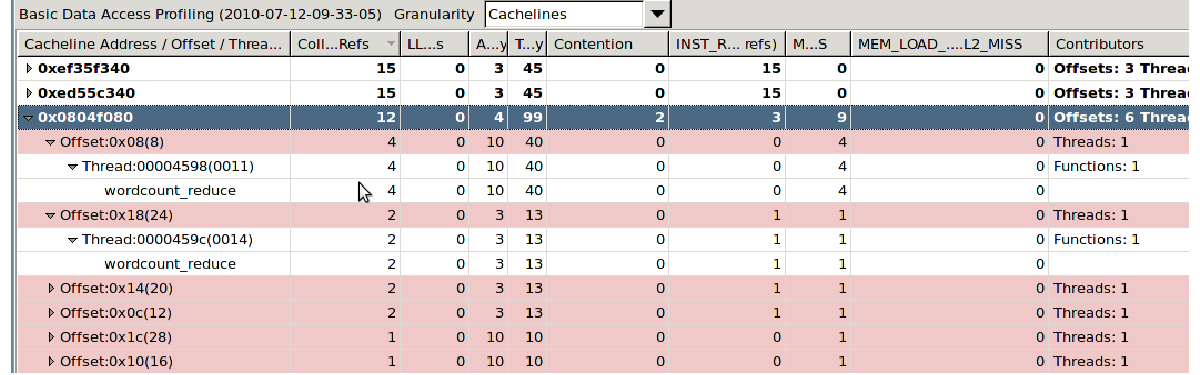
\includegraphics[width=6in]{figure/wordcount}
\caption{PTU output for \texttt{word\_count}.
\label{fig:wordcount}}
\end{figure*}

It should take a lot of effort to find the problem since PTU only present functions using 
one cache line, not to mention that PTU can report huge numbers of false sharing cache lines.
Another shortcoming of PTU is that ``Collected Data Refs'' number cannot be used a metrics 
to evaluate the significance of false sharing problems. For this example, PTU only reports 
12 times references (13767 times for Sheriff). 
%That is why we cannot relying on PTU to do the analysis of false sharing
%problems given the large number of cache lines involved. 

\subsection{Performance of Sheriff}
\label{sec:results-runtime-overhead}

\begin{figure*}[!t]
\centering
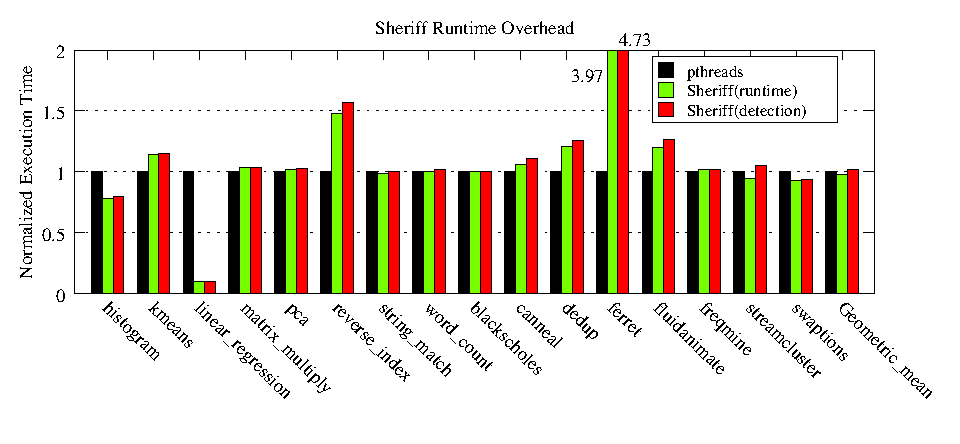
\includegraphics[width=6in]{figure/performance}
\caption{Runtime overhead for Sheriff across a suite of benchmarks,
  normalized to the performance of the pthreads library (see
  Section~\ref{sec:results-runtime-overhead}). Sheriff incurs little
  overhead for two multithreaded benchmark suites.
\label{fig:overhead}}
\end{figure*}
We have evaluated Sheriff on two multithreaded benchmarks suites, Poenix and PARSEC. 
The results can be seen from Fig.~\ref{fig:overhead}. 
There are two outliers in the results. One is \texttt{linear\_regression}, 
it shows almost 10X speedup against the one using pthreads library. 
There is a serious falsesharing problems inside (see Table~\ref{table:perfafterfix}), the runtime system
Sheriff relying on can avoid this type of false sharing problem (long transaction, without synchronization inside)
automatically. Even the sampling mechanism added to capture continous interleaving writes can add little overhead
on that, we can still achieve significant performance benefit. 
Another outlier is ferret benchmarkd of PARSEC suite. The performance overhead of Sheriff on this benchmark
is about 4.97X slower than the one using pthreads libarary. 

In order to find out what can affect the performance of Sheriff, we listed some charecteristics about these 
evaluated benchmarks in Table~\ref{table:characteristics}.
According to our analysis, the following parameters can affect the performance of Sheriff. 
\begin{itemize}
\item
Pages written: each write on one protected page should pay some additional overhead 
to un-protect the page in the page fault handler. 
Then in the sampling handler Sheriff should check cache writes for each shared written page and in the 
end of transaction Sheriff should check cache writes for each page and commit the modification to shared space. 

\item
Transaction length: Sheriff introduces some overhead in the beginning of transaction and in the end of each 
transaction. Longer transaction is expected to amortize the overhead. 

\item 
Allocation times: Sheriff should attach callsite for every allocations, thus should pay a little overhead on every allocation.

\item
Cache cleanup size: Sheriff cleanup the invalid cache counting information in the memory allocation 
if one allocation is involving in the re-usage of memory of those freed memory objects. In the actual implementation,
since there is no cache counting information when there is one thread (memory are protected when the first thread are spawned)
only those allocations after memory are protected (see Section~\ref{discussion-perf}) needs to be cleaned their cache counting
information to improve the performance.
\end{itemize}

From the results from Table~\ref{table:characteristics}, we can confirm our analysis. 
Allocation times and Cache cleanup size didn't affect the performance greatly. 
When pages number written is large, that will affect the performance.
Especially when average pages written on one unit time is large, that can affect the performance greately.
Fig.~\ref{fig:overhead} shows that Sheriff's performance are affected greately 
on benchmarks \texttt{ferret}, \texttt{reverse\_index}, \texttt{dedup} and \texttt{fluidanimate}, 
characteristics showed in Table~\ref{table:characteristics} that the first three benchmarks 
have a very high \textbf{PagesPerMs}. That is, every microsend 
needs to handle protected pages are pretty high in these three benchmarks. 
\texttt{fluidanimate} is an outlier if we are just using the \textbf{PagesPerMs} metrics. 
The reason of \texttt{fluidanimate } with a high overhead is that there are huge amounts of transactions inside (about 10M). 
When we checked the source code, we found that there are a lot of \texttt{mutex\_lock()}
and \texttt{mutex\_unlock()} calls in this application.
Remember that we have done some modifications on synchronization function calls, every time we have to get actual 
synchronization variables from ``nominal variable'', huge amounts of these operations bring us some overhead on this benchmark.
In fact, \texttt{ferret} have most of attributes that can affect performance, huge amounts of pages (about 3.45G data) and huge 
amounts of transactions (avout 1M). That is why \texttt{ferret} runs really slow on Sheriff.
But that should not be the attributes of most of multithreaded applications.

\begin{table*}
\centering
\begin{tabular}{|l|rrrr|rr|r|}
\hline
{\bf \small Benchmark} & {\bf \small PagesWritten} & {\bf \small Commits} & {\bf Allocs} & {\bf \small CleanupSize} & {\bf \small TranLength(ms)} & {\bf \small PagesPerTran} & {\bf \small PagesPerMs}\\
\hline
\small \textbf{histogram} & 0 & 24 & 2 & 0 & 12.5 & 0 & 0\\
\small \textbf{kmeans} & 1312 & 3836 & 101002 & 0 & 4.15 & 0.34 & 0.08\\
\small \textbf{linear\_regression} & 16 & 24 & 3 & 0 & 38.6 & 0.67 & 0.02\\
\small \textbf{matrix\_multiply} & 16 & 24 & 11 & 0 & 313.23 & 0.67 & 0.0\\
\small \textbf{pca} & 0 & 47 & 2 & 0 & 450.69 & 0 & 0.0\\
\small \textbf{reverseindex} & 260201 & 156409 & 250927 & 0 & 0.05 & 1.66 & 30.99 \\
\small \textbf{string\_match} & 0 & 24 & 7 & 0 & 104.75 & 0 & 0.00\\
\small \textbf{word\_count} & 145 & 89 & 38 & 32 & 25.08 & 1.63 & 0.06\\
\hline
\small \textbf{blackscholes} & 0 & 23 & 4 & 0 & 453.51 & 0 & 0.0\\
\small \textbf{canneal} & 8 & 1056 & 5974612 & 0 & 10.32 & 0.01 & 0.0\\
\small \textbf{dedup} & 76184 & 45636 & 8291 & 0 & 0.04 & 1.67 & 44.9\\
\small \textbf{ferret} & 904381 & 1072258 & 110558 & 0 & 0.01 & 0.84 & 76.04\\
\small \textbf{fluidanimate} & 8 & 10018550 & 135430 & 352 & 0.00 & 0.00 & 0.00\\
\small \textbf{freqmine} & 0 & 1 & 33 & 0 & 11524.6 & 0 & 0.0 \\
\small \textbf{streamcluster} & 32824 & 128557 & 12 & 294 & 0.02 & 0.26 & 10.42\\
\small \textbf{swaptions} & 48 & 24 & 388 & 0 & 167.23 & 2 & 0.01\\
\hline
\end{tabular}
\caption{Characteristics of benchmarks. 
\label{table:characteristics}}
\end{table*}

%%%%%%%%%%%%%%%%%%%%%%%%%%%%%%%%%%%%%%%5
%%%% Some data to list the effectiveness of this tool.
%%%%%% How many caches are carried for each test case. 
%%%%%% Whether all caches has false sharing problem.
%%%%%%%%%%%%%%%%%%%%%%%%%%%%%%%%%%%%%%%

